\chapter{PGP / Gnu Privacy Guard}
Pretty Good Privacy (PGP) pada awalnya adalah aplikasi yang dapat digunakan
pengguna untuk menggunakan kriptografi di berbagai aplikasi dengan lebih mudah.
Pengembangan selanjutnya PGP menjadi bagian dari {\em public key
infrastructure}.

\section{Sejarah}
[... more to be written ...]

Gnu Privacy Guard (GPG) merupakan implementasi dari PGP yang bersifat terbuka.
(Catatan: Singkatan dari GPG ini merupakan guyonan terhadap PGP.) Bab ini akan
membahas lebih banyak tentang GGP, meskipun konsep yang sama dapat juga
diterapkan pada PGP jika Anda menggunakan produk PGP yang komersial.

Dalam buku ini, kita akan menggunakan GPG versi {\em command line interface},
yaitu dengan mengetikkan perintah ``gpg'' di program terminal atau CMD.exe.
Ada banyak program {\em GUI} dari GPG ini. Silahkan gunakan manual terkait
dengan program-program tersebut. Prinsipnya masih tetap sama.

\section{Menggunakan Gnu Privacy Guard, gpg}
Awal dari penggunakan GPG adalah membuat pasangan kunci publik dan privat. Hal
ini dapat dilakukan dengan menggunakan perintah berikut.

\begin{verbatim}
gpg --key-gen
\end{verbatim}

Perintah di atas akan menanyakan beberapa hal, seperti jenis algoritma yang
digunakan (pilih RSA dan RSA), panjang kuncinya (pilih 2048), dan alamat email
yang akan digunakan untuk kunci tersebut. Dalam contoh buku ini saya akan
menggunakan alamat email ``rahard2017@gmail.com''. Gunakan alamat email Anda
sebagai penggantinya/

\begin{verbatim}
$ gpg --gen-key
gpg (GnuPG/MacGPG2) 2.0.30; Copyright (C) 2015 Free Software Foundation, Inc.
This is free software: you are free to change and redistribute it.
There is NO WARRANTY, to the extent permitted by law.

Please select what kind of key you want:
   (1) RSA and RSA (default)
   (2) DSA and Elgamal
   (3) DSA (sign only)
   (4) RSA (sign only)
Your selection? 1
RSA keys may be between 1024 and 4096 bits long.
What keysize do you want? (2048)
Requested keysize is 2048 bits
Please specify how long the key should be valid.
         0 = key does not expire
      <n>  = key expires in n days
      <n>w = key expires in n weeks
      <n>m = key expires in n months
      <n>y = key expires in n years
      Key is valid for? (0) 3m
Key expires at Wed May 31 10:30:37 2017 WIB
Is this correct? (y/N) y

GnuPG needs to construct a user ID to identify your key.

Real name: Budi Rahardjo
Email address: rahard2017b@gmail.com
Comment:
You selected this USER-ID:
    "Budi Rahardjo <rahard2017@gmail.com>"

Change (N)ame, (C)omment, (E)mail or (O)kay/(Q)uit?
\end{verbatim}

Setelah proses {\em key generation} selesai, kunci publik dapat diekspor dengan
menggunakan perintah  berikut. Gantikan ``rahard2017@gmail.com'' dengan alamat
email Anda.

\begin{verbatim}
gpg --export --armor rahard2017@gmail.com > kunci-public.asc
\end{verbatim}

Akan dihasilkan berkas ``kunci-public.asc''. Tanpa perintah {\em redirect
output} yang menggunakan ``>'' itu, hasilnya hanya akan ditampilkan di layar
saja. Tentu saja Anda dapat menggunakan nama berkas lainnya.
Berikut ini adalah contoh beberapa baris pertama dari berkas ASCII hasil ekspor
kunci tersebut. (Tampilan bisa panjang sekali, bergantung dari panjang kunci
yang digunakan.)

\begin{verbatim}
-----BEGIN PGP PUBLIC KEY BLOCK-----
Comment: GPGTools - https://gpgtools.org

mQENBFiiijUBCAD3ZIxjUQyDtcGTmHs2iU+2aS+MMp2w+codVRrqLfVI+V8S+TmP
WGe2Gu4pTLovGzZ2NGWvKACZ0A+BL97e9K6QN6+UIYRArFdxfojQ4lbwH/WO1YSn
J6BsCE1IfX8niRiskdibBhZZcrUCcDa/tgvgXTymoAeZEcMwR48hEOUWuOGoCE2g
TA/kD9yCyorFUKEsbyKJMKPtlMJGICUwtggDdXT5arCCafpydLGxok+w4TJjADeX
jeTxDgYSNjCNar9wRhtnG+G/Irbfctj77/9Ppz8j8Dp1NkAwx5P+9AJRNNkwU88c
7FSEz0cpAzgC4VyaL/iX85G8wr6z5kaWNV3FABEBAAG0JEJ1ZGkgUmFoYXJkam8g
PHJhaGFyZDIwMTdAZ21haWwuY29tPokBPQQTAQoAJwUCWKKKNQIbAwUJABuvgAUL
...
\end{verbatim}

Kunci publik ini yang akan didistribusikan secara publik, misal disimpan di
blog Anda. Kunci ini juga dapat disimpan di {\em key server}.

Untuk melihat informasi mengenai kunci Anda, dapat digunakan perintah berikut:

\begin{verbatim}
gpg --fingerprint rahard2017

pub   2048R/EB6CEB46 2017-02-14 [expires: 2017-03-07]
      Key fingerprint = 810B 2149 3366 E699 F95E  9E49 07E1 BDC5 EB6C EB46
uid       [ultimate] Budi Rahardjo <rahard2017@gmail.com>
sub   2048R/C2E83C60 2017-02-14 [expires: 2017-03-07]
\end{verbatim}

Perhatikan bahwa kunci publik yang ini memiliki ID ``EB6CEB46''. ID ini dapat
digunakan untuk bertukar kunci, atau untuk melakukan proses-proses lainnya.
Sebagai contoh, kita dapat mengirimkan kunci ini ke server agar dapat dilihat
atau dicari oleh orang lain. Keyserver yang akan kita gunakan dalam contoh ini
adalah pgp.mit.edu.

\begin{verbatim}
gpg --keyserver pgp.mit.edu --send-keys EB6CEB46
\end{verbatim}

Pengirimkan kunci dapat juga dilakukan dengan menggunakan web dari situs PGP
MIT tersebut sebagaimana dicontohkan dalam gambar berikut. Masukkan teks ASCII
kunci Anda ke kolom kunci dan upload.

\begin{figure}[ht]
\fbox{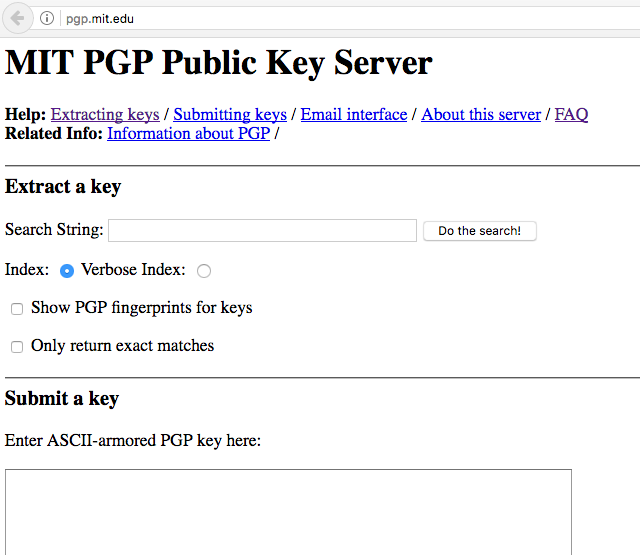
\includegraphics[width=1.0\linewidth]{graphics/pgp-mit.png}}
\caption{Key server pgp.mit.edu}
\label{fig:pgp-mit}
\end{figure}


\begin{mdframed}[backgroundcolor=blue!20] 
\begin{ExerciseList}
   \Exercise[title=Membuat Kunci]
   \Question{Buat pasangan kunci publik dan kunci privat Anda. Gunakan parameter
   default saja (RSA dan RSA). Asosisasikan dia dengan alamat email Anda.} 
   \Question{Unggah kunci publik Anda ke salah satu keyserver yang tersedia 
   (misal pgp.mit.edu atau keyserver.cert.or.id)} 
   \Question{Beritahukan teman-teman Anda tentang kunci Anda tersebut. Minta
   mereka untuk ikut menandatangani kunci publik Anda tersebut.}
\end{ExerciseList}

\end{mdframed}

\subsection{Enkrip Untuk Sebuah Alamat Email}
Salah satu fungsi dari PGP/GPG adakan mengirim pesan secara rahasia. Pesan
tersebut dienkrip dengan menggunakan kunci publik (alamat email) tujuan.
Sebagai contoh, kita akan mencoba mengirimkan pesan rahasia ke
rahard2017@gmail.com.

Langkah pertama tentunya kita harus mendapatkan kunci publik dari akun email
rahard2017 tersebut. Cari di salah satu keyserver, unduh, dan masukkan ke
gantungan kunci kita.

\begin{verbatim}
gpg --keyserver hkp://pgp.mit.edu --search-keys rahard2017
\end{verbatim}

Dalam contoh ini, kita akan menggunakan berkas ``dokumen.txt'' yang berisi
pesan dalam bentuk {\em plain text}. Tentu saja PGP/GPG tidak membatasi jenis
pesan (berkas). Dalam contoh ini saja kita akan menggunakan berkas teks yang
berisi teks ASCII. Secara umum berkas biner (MS Word, lagu MP3, film MP4, dan
seterusnya) dapat juga diproses. Isi berkas dokumen.txt tersebut adalah sebagai
berikut.

\begin{mdframed}[backgroundcolor=blue!20] 
\begin{verbatim}
Ini adalah dokumen untuk percobaan menggunakan PGP/GPG.
Untuk tanda tangan, isinya tidak harus disembunyikan.
Selamat mencoba.
\end{verbatim}
\end{mdframed}

Perintah untuk mengenkripsi dengan menggunakan kunci publik tujuan
(rahard2017@gmail.com) adalah seperti dicontohkan di bawah ini. Perintah
tersebut akan menghasilkan berkas ``dokumen.pgp''.

\begin{verbatim}
gpg --output dokumen.pgp --encrypt --recipient rahard2017@gmail.com dokumen.txt
\end{verbatim}

Berkas ``dokumen.pgp'' yang dihasilkan dari proses enkripsi di atas berupa
berkas biner. Jika kita ingin menghasilkan berkas dalam bentuk ASCII, maka
gunakan opsi ``-armor'' (-a) seperti perintah di bawah ini.

\begin{verbatim}
gpg -a --output dokumen.pgp --encrypt --recipient rahard2017@gmail.com dokumen.txt
\end{verbatim}

Jika kita lihat berkas ``dokumen.pgp'', isinya adalah seperti berikut.

\begin{mdframed}
\begin{verbatim}
-----BEGIN PGP MESSAGE-----
Comment: GPGTools - https://gpgtools.org

hQEMAy/vbaXC6DxgAQf/Zjk74t1FXTT3abmJUz/w5Z8iHIIEWZlvMmBdMS7w/2U8
L2NvrvG6GOrsduLTIrybCIAQ0GPU9Nq+YOMYJaY3BhiqkCSyYhHYRk0406OS3GCA
ONnhiqKiVLJIyfNWdDBtB4k7s8pfM5ngxgeZ6/gH5TDspHrhjrLS65Stn7sr+Nlf
TSuG9p21vr19yL13KBkd2rI5WBnL68/3bRJnKt0JL1PLeMvQ0eZIiRXcmropPXIs
rltFRflpdp0H0LJn2/xQ5rXr13QRRjzo3SL4i/eYxPlEmpD164aicI8LC+qKgYcc
FShUuTxwxtu7tPYpqEH17jTTd29wZdrXDFHp5TGLTdKtAeMKeGupxvicOaNMY46J
S3LBC9fU2bywwmvM77cCr97DOP1rA6WXR2xluRvLhms83lNMcpSDuZCPpb8rxKmu
Xk2WFThfV5rq0I1kyP2Kc1g+0cgnJkAzFXe5MQRIOpJ/MRwrekAo3Dvp3TefwMYu
R3LYwCi8VstPpnH9rcFyoyxsqMqLTPtUnheISNUmVERtLm3rALtHjf2vyvkR/2JF
Vmu79aqbbFJPJZ0gNmk=
=D+3L
-----END PGP MESSAGE-----
\end{verbatim}
\end{mdframed}

Berkas ``dokumen.pgp'' tersebut dapat kita kirimkan (misal melalui email) ke
rahard2017@gmail.com. Di sisi penerima (rahard2017), berkas tersebut dapat dia
buka dengan menggunakan kunci privatnya. Ketika menggunakan kunci privat,
biasanya pengguna ditanyakan {\em passphrase} untuk mengakses (membuka) kunci
privat tersebut karena biasanya kunci privat dilindungi dengan {\em passphrase}
tersebut.

\begin{mdframed}
\begin{verbatim}
gpg --decrypt dokumen.pgp

You need a passphrase to unlock the secret key for
user: "Budi Rahardjo <rahard2017@gmail.com>"
2048-bit RSA key, ID C2E83C60, created 2017-02-14 (main key ID EB6CEB46)

gpg: encrypted with 2048-bit RSA key, ID C2E83C60, created 2017-02-14
      "Budi Rahardjo <rahard2017@gmail.com>"
Ini adalah dokumen untuk percobaan menggunakan PGP/GPG.
Untuk tanda tangan, isinya tidak harus disembunyikan.
Selamat mencoba.
\end{verbatim}
\end{mdframed}

Seperti dilihat pada contoh di atas, teks aslinya ditampilkan di layar. Jika
kita ingin menyimpannya ke dalam sebuah berkas, maka dapat kita gunakan opsi
``--output namaberkas'' ketika menjalankan perintah gpg tersebut di atas.

Perlu diingat kembali bahwa hanya orang yang memiliki kunci privat, yaitu
rahard2017@gmail.com, yang dapat membuka berkas tersebut. Jika berkas tersebut
dicoba untuk dibuka dengan kunci lain, maka dia tidak dapat menghasilkan isi
yang sama.

\subsection{Tanda Tangan Dokumen}
Salah satu manfaat penggunaan PGP/GPG adalah tanda tangan digital (sign). Dalam
contoh berikut ini kita akan mendatangani berkas ``dokumen.txt''. (Kita dalam
contoh ini adalah ``rahard2017@gmail.com''.)

\begin{verbatim}
gpg -u rahard2017@gmail.com --output dokumen.sig --sign dokumen.txt

You need a passphrase to unlock the secret key for
user: "Budi Rahardjo <rahard2017@gmail.com>"
2048-bit RSA key, ID EB6CEB46, created 2017-02-14
\end{verbatim}

Seperti sebelumnya, berkas yang dihasilkan (dokumen.sig) dalam format biner.
Untuk menghasilkan berkas ASCII, dapat digunakan ``-a''.

\begin{verbatim}
gpg -a -u rahard2017@gmail.com --output dokumen.sig --sign dokumen.txt
\end{verbatim}

Isi berkas ``dokumen.sig'' yang sudah di-armor-kan seperti ini. Sebagai
catatan, isi dokumen dan tanda tangan tercampur dan ter-armor-kan. Kerugian
cara ini adalah isi dari dokumen tidak dapat terlihat secara langsung.

\begin{verbatim}
-----BEGIN PGP MESSAGE-----
Comment: GPGTools - https://gpgtools.org

owGbwMvMwMXI/nDv0dc5r90Y10xI4k7Jzy7NTc3TK6koidipudUzL1MhMSUxJzFD
ASqjUJpXUpqtUJBalJyflJiYpwAUS08vzUvMBrID3AP03QPc9bhCwYpKEvNSEkFk
emKejkJmcWZeJZCbmZKYrZCRWFRarJCSWZyam1SaV5kJ1K3HFZyak5ibWAIyEmS4
HlcnowwLAyMXAxsrE8g1DFycAjDXcoix//d7pfhQ+pbBxM4ilx/pi054OOkFsfS2
TDDSVY/Zec58cp/zm9TgDczKn+71Kkqvs/4fNNvRuUr208VdwowLPTliFpR+O2/L
0cR/KDTuie6h9Xlq3bXTSg6kpeoxblZ323ra4jDfvvs/9RjeSByS0cp4+T/c81B6
YUepNtO0hLjZZeGxR63yNqxbu7ZX9djt4p6a7/JTbJKepvo3XItlO8x0xVDt3LIv
oRc/tc7667WqskaC95zr1E6xREHL5eEKGnkByy7arEnL0Ge++bNd4ET4NOV3FYqP
L875kT8v8PeVPdqr+SrENG7YNL6+PWXOvNUR6ruMVdSOhzEoeyn4P2EWX6J1dVL/
n1dzXzdrAgA=
=VRfS
-----END PGP MESSAGE-----
\end{verbatim}

Ada cara untuk memisahkan isi (teks) dan tanda tangannya. Perintah yang
digunakan adalah ``--clearsign''.
\begin{verbatim}
gpg -u rahard2017@gmail.com --output dokumen.sig --clearsign dokumen.txt
\end{verbatim}

Hasilnya adalah sebuah berkas yang isinya adalah sebagai berikut. Perhatikan
bahwa isi dan tanda tangan terpisah, meskipun masih dalam sebuah berkas.

\begin{mdframed}[backgroundcolor=red!20]
\begin{verbatim}
-----BEGIN PGP SIGNED MESSAGE-----
Hash: SHA512

Ini adalah dokumen untuk percobaan menggunakan PGP/GPG.
Untuk tanda tangan, isinya tidak harus disembunyikan.
Selamat mencoba.
-----BEGIN PGP SIGNATURE-----
Comment: GPGTools - https://gpgtools.org

iQEcBAEBCgAGBQJYuSthAAoJEAfhvcXrbOtG1pkIALaFxIxKObM7p/ZTMpzNCIHN
GpyR9Q6QQEi+9+0loHdw1TqMEskJ3HxWOnegupMueiIpO0IaEd8qCraLSfRF3G1f
gBxl837rXnTjDIYABN9T6f5GrZHyeWXEhwDRDuLWsb9v85pNd/RUbQ8L7N/s4SUl
NgyPbHKhal+ob047mHE1zF9lvpuRfhWM3ztr8OJN6MWTgb+NYpc0b9YuyqSRiDZ0
y3fvY3iRexMjLI2dxhXOTWG4IM5ouwbFtheJML1Lssh/pn1KZwicnWGAouWhQTOY
hGR8zSoy4oeS/hlUmdAu3bse73pcWeybCtYLwvXSBvg7W67sCOERmIfZxXxtq08=
=/uVR
-----END PGP SIGNATURE-----
\end{verbatim}
\end{mdframed}

Untuk melakukan verifikasi apakah dokumen tersebut terjamin integritasnya
(isinya tidak berubah dan yang menandatangani benar), gunakan perintah
``verify''.

\begin{mdframed}
\begin{verbatim}
gpg --verify dokumen.sig
\end{verbatim}
\end{mdframed}


Seringkali ada kebutuhan untuk memisahkan berkas dari tanda tangan dan
dokumennya. Sebagai contoh, jika dokumen yang ingin kita tandatangani adalah berkas
biner (dokumen {\em word processor}, audio, video, dan sejenisnya), maka tanda
tangan dan dokumennya harus dipisah.

\begin{verbatim}
gpg -u rahard2017@gmail.com --output dokumen.sig --detach-sig dokumen.txt
\end{verbatim}

Untuk melakukan verifikasi bahwa dokumen tersebut benar (isinya benar dan yang
menandatangani benar juga) jika dokumennya dipisah adalah sebagai berikut.

\begin{mdframed}
\begin{verbatim}
gpg --verify dokumen.sig dokumen.txt
\end{verbatim}
\end{mdframed}

\begin{mdframed}[backgroundcolor=blue!20]
\begin{ExerciseList}
   \Exercise[title=Verifikasi]
   \Question{Menurut Anda, apakah tanda tangan (signature) akan tetap sama
   untuk setiap orang meskipun dokumen yang ditandatangani berbeda-beda?
   Ataukah untuk dokumen yang berbeda, tanda tangan digital dari dokumen 
   tersebut akan berbeda?}
   \Question{Verifikasi dokumen dengan data yang benar. Maksudnya jangan ubah
   berkas ``dokumen.sig'' dan ``dokumen.txt''.}
   \Question{Verifikasi dokumen dengan data yang sudah tercemar. Edit berkas
   dokumen.txt sehingga berbeda dengan aslinya. Coba verifikasi. Tunjukkan
   bahwa proses verifikasi gagal.}
\end{ExerciseList}
\end{mdframed}

\section{Tools}
Perintah-perintah dalam contoh pada bagian sebelumnya dilakukan dengan
menggunakan {\em command line}. Ada beberapa {\em tools} (biasanya memiliki
{\em graphical user interface}) yang dapat membantu untuk mempermudah operasi.
{\em Tools} yang tersedia bergantung kepada sistem operasi yang Anda gunakan. 


\section{Web of Trust}
Keamanan dari PGP/GPG ini berbasis {\em web of trust}. Bagaimana kita dapat
mempercayai bahwa kunci publik tersebut milik dari ``Budi Rahardjo'' dengan
alamat email tersebut (rahard2017@gmail.com)? Boleh jadi ada seseorang yang
dengan sengaja memalsukan identitas tersebut. 

Proses verifikasi dilakukan oleh orang lain dengan menandatangani kunci
tersebut dan kemudian data tersebut - kunci yang sudah ditandatagani - diunggah
kembali ke keyserver. 
